
 \vspace{0.5cm}
 
 The previous chapters detailed the proposed methodology for network inference from incomplete abundance data. The species abundances $\Ybf$ are jointly modeled in a GLMM using the Poisson log-normal distribution, thus taking advantage of its properties to account for offsets and experimental and/or environmental covariates $\Xbf$. The problem of network inference is then transposed to the Gaussian latent layer of model parameters $\Zbf$, where it is performed using averaging on spanning-tree structures with decomposable distribution on trees parametrized with edges weights $\betabf$. Missing actors are inferred in the Gaussian layer as well, simultaneously with the network. We remind the mathematical formulation of this model:
  \begin{equation*}
 \left\{ \begin{array}{l}
 \begin{array}{ll}
 T\sim \prod_{kl\in T} \beta_{kl} / B, &B= \sum_{T\in\mathcal{T}} \prod_{kl \in T} \beta_{kl},\\\\
 \Zbf_i\mid T  \sim \Ncal (0, \Omegab_T), &\{\Zbf_i\}_i \text{ iid, }\\
 \end{array} \\\\
 Y_{ij}\mid \Zbf_i\sim \Pcal (\exp (o_{ij}+\xb_i^\intercal \thetab_j + Z_{ij})), \; (Y_{ij} \independent) \mid \Zbf_i .
 \end{array} \right. 
 \end{equation*}
 
 The qualities of this approach have been demonstrated on simulated examples as well as empirical datasets. But why does it work ? Mostly because exact computations are possible in the Gaussian layer, thanks to its maniability and the structure and algebraic properties of spanning trees.  This flexibility calls for some natural extensions which were not developed due to time constraints, that we now present together with specific details of this model.
 
 
\section{Unresolved questions}
\subsubsection*{Offset modeling}
The presented methodology allows to take into account covariates and offsets, which is paramount in the modeling of experiments. A change in the covariates included can greatly modify the inferred network, however this is an information that can be controlled. On the other hand, not including offsets amounts to model incoherent data and therefore yields inconsistent results. Unfortunately, offsets are not always obvious or easy to get, and evaluating them possibly represents a modeling step in itself. For example in an ecological census of fauna, the offset has to at least account for the period of time of observation, the experience of the observer and the species detectability, which is obviously the most difficult to get. Detectability depends on the relative position of the species to the observer, and can depend on the environmental conditions as well, making its modeling a delicate step.\\

\subsubsection*{Algorithm initialization}
The approach can also infer missing actors as detailed in Chapter 3. The initialization of the algorithm for this inference requires an initial clique of neighbors for each missing actor. This parameter is critical, as it defines all the initialization and if it is too far from the true clique, that is if not a minimum of true neighbors are included, the procedure can degenerate and abort. Several methods for setting this parameter are proposed in the nestor package. They are based on finding groups of highly correlated variables (sparse PCA and model-based clustering of the estimated correlation matrix), or finding clusters in the structure of the marginal graph (using Stochastic Bloc Models). The estimated lower bound of the likelihood can be used to choose between a large set of results with different initializations, thus one way to go is simply to sample several starting points (possibly by boostrapping the previous methods) and test all of them. Many other methods could be used, as well as prior knowledge on species, and we do not conclude on the best way to initialize the cliques. However we observed that it is less important for the inference quality to be precise than to include some true neighbors in the clique. Therefore we advise to choose the initial clique also based on its size.\\

\subsubsection*{Model selection}
One key question when working with possibly incomplete data is to know if it is indeed incomplete, and to what extent. This amounts to model selection to chose the number of missing actors $r$.  Usually model selection is carried out with computations on the likelihood of each model. The model developed involves several latent parameters, and the inference is therefore performed in a variational framework which yields a lower bound of the likelihood. Moreover as the method takes advantage of the variational estimation of the PLN model described in \citet{CMR18}, the quantity that is computed is actually an approximation of this lower bound. This results in the usual model selection tools, which originally apply to likelihoods, to not work (Akaike/Bayesian/Extended Bayesian Information Criterion). Then the only strategy left is to resort to cross-validation, which is greedy and not very satisfying either. There is a need of  adapted criteria for  models with variational inference, which is still an open research question of statistical theory.

\section{Extensions of the adopted approach}
In this section, we present direct extensions of the developed methodology regarding the network in itself (estimation of its parameters, network comparison), and the data nature (processing of different data types and spatialized data).
\subsection{Characterizing species interactions}


Generally, species interactions are characterized by their sign and strength. This information is contained in  the partial correlation matrix, defined as $\Rbf_p=(\rho_{jk})_{1\leq j,k\leq p}$ with $$\rho_{jk}=\frac{-\omega_{jk}}{\sqrt{\omega_{jj}\omega_{kk}}},$$
 which is simply the opposite of the correlation matrix built from the precision matrix $\Omegabf$. Some methods are thus dedicated to the estimation of the partial correlation matrix to build knowledge on an ecosystem functioning. In the context of Gaussian Graphical Models, \cite{Lau96} develops maximum likelihood estimators for the precision matrix which depends on that of the covariance matrix, and the structure of the graph, as detailed in section \ref{ggm:mle}. It thus requires the precise knowledge of the graph, and even more than that: the only terms of the covariance matrix that are correctly estimated are those corresponding to edges in the graph. Therefore the prior inference of the structure is necessary. Moreover, these MLE are only valid for decomposable graphs, therefore using Proposition \ref{decomp} the network might need to be triangularized as illustrated in Figure \ref{chordal}. Therefore following these three steps: 
\begin{enumerate}
\item Infer the conditional dependency structure $\G$,
\item Make $\G$ a chordal graph,
\item Compute $\widehat{\Omegabf}_{MLE}$.
\end{enumerate}
 would lead to an approximation of $\Omegabf$. Note that there is not a unique solution to step 2.  If the inferred network is already chordal, this  yields  the MLE of $\Omegabf$, available after the network inference.

\begin{figure}
\centering
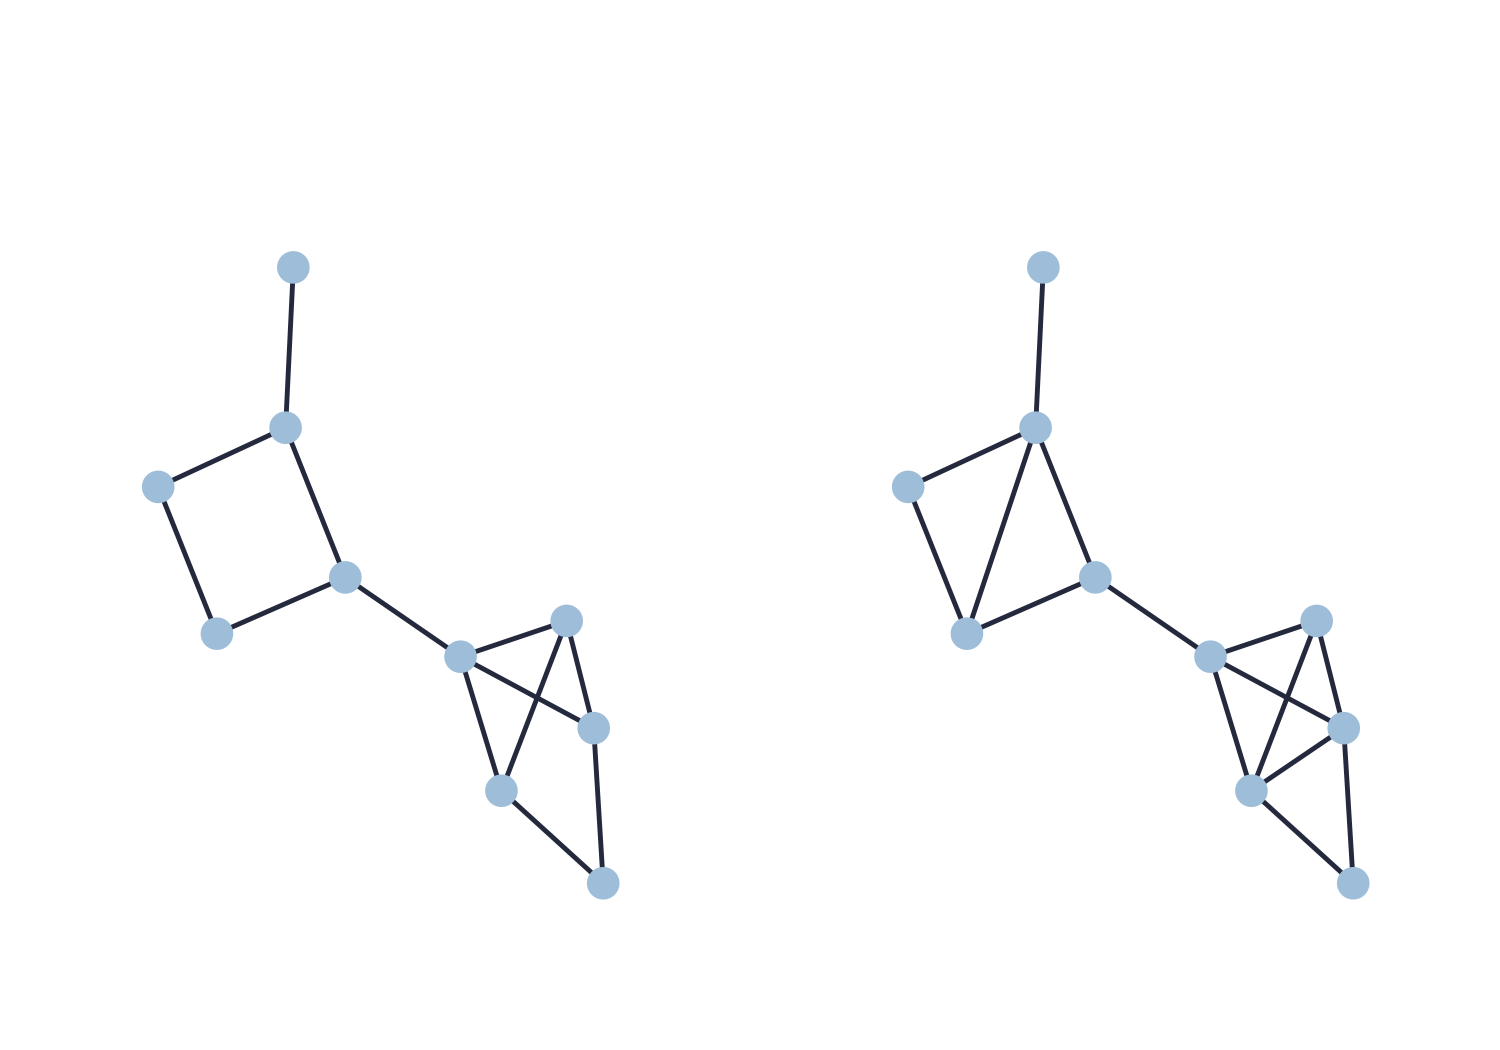
\includegraphics[width = 0.6\linewidth]{figs/chordal.png}
\caption{Example of triangularization. \textit{Left}:  graph $\G$. \textit{Right}: a chordal version of $\G$: maximal loops are of size 3.}
\label{chordal}
\end{figure}
\subsection{Network comparison}
 
Comparing networks has many applications and  yields results of interest in various fields, regarding for example the evolution of a system across seasons, or how a pathogen modifies the organization of a microbiome.

The comparison from a statistical point of view is linked to testing differences, or questioning the independence of two networks for example.  Rather than defining statistical tests based on networks distributions, current strategies consists in summarizing networks with vectors of measures on nodes. These are called embeddings, which aim to capture the structure of the graph and the relationships between the nodes in a concise manner (e.g. \citet{TMK18,CK19}). Embeddings can then be compared using PCA for example. The presented approach assumes the graph is a latent tree, which estimated distribution can be seen as another available graph summary.\\

A first step toward statistical network comparison using trees could be to compare the estimated laws on trees, for example using the Küllback-Leibler divergence which is easily written with tree distributions and gives two interesting quantities.

First, it is possible to compute the contribution of a specific edge $kl$ to the distribution. We denote $p_{\betabf_{\setminus kl}}$ the  decomposable tree distribution where the weight $\beta_{kl}$ is set to zero. Its normalization constant is  $B_{\setminus kl}=\sum_{T\in\mathcal{T}} \prod_{uv\neq kl} \beta_{uv}$. Computing the Küllback-Leibler divergence between $p_\betabf$ and $p_{\betabf_{\setminus kl}}$ yields  the contribution of $kl$ to $p_\betabf(T)$. It writes:
\begin{align*}
KL( p_\betabf (T)\mid\mid p_{\betabf_{\setminus kl}} (T)) &= \Esp_{p_\betabf (T)} [\log p_\betabf (T) - \log p_{\betabf_{\setminus kl}} (T)]\\
&=P_{kl} \log \beta_{kl} + \log ( B_{\setminus kl}/B).
\end{align*}
Where $P_{kl} = \Esp_{p_{\betabf}}[\mathds{1}\{kl\in T\}]$ is the probability for the edge $kl$ to be in tree $T$ under the tree distribution $P_{\betabf}$. Now noticing that $B_{\setminus kl}/B=1-P_{kl}$, we finally get the following contribution of $kl$:
$$KL( p_\betabf (T)\mid\mid p_{\betabf_{\setminus kl}} (T)) =P_{kl} \log \beta_{kl} + \log (1-P_{kl}).$$
%peut être utile pour ordonner les arêtes par importance si trop de probabilités égales. Besoin de faire un test pour voir si la qté existe 	vec une proba à 1 (existance de B\kl)
As the distribution under which the expectation is taken must be dominant over the other, the divergence $KL(p_{\betabf_{\setminus kl}} (T)\mid\mid p_\betabf (T)) $ is not defined.

Then, if all edges weights are finite and non-null, the divergence can be symmetrized into a so-called dissimilarity measure to compare two networks. Assuming the data is observed under two conditions $A$ and $B$, we consider the edges weights matrices estimated from each subsets $\betabf^A$ and $\betabf^B$. The dissimilarity measure between the tree distributions  $p_{\betabf^A}(T)$ and $p_{\betabf^B}(T)$ writes:
\begin{align*}
D(p_{\betabf^A}(T), p_{\betabf^B}(T)) &=\frac{1}{2} \left[KL\big( p_{\betabf^B} (T) \mid\mid p_{\betabf^A}(T)\big)+KL\big( p_{\betabf^A}(T)\mid\mid p_{\betabf^B} (T)  \big)\right].
\end{align*}
After computation, this actually simplifies into the following expression, where $P_{kl}^A = \Esp_{p_{\betabf^A}}[\mathds{1}\{kl\in T\}]$ is the probability for the edge $kl$ to be in tree $T$ under the tree distribution $p_{\betabf^A}$:
$$D(p_{\betabf^A}(T), p_{\betabf^B}(T)) = \sum_{kl} \log (\beta_{kl}^A /\beta_{kl}^B) \left( \frac{P_{kl}^A - P_{kl}^B}{2}\right).$$

Finally if we consider $K$ different conditions,  the $K$ tree distributions could be compared by computing the $K\times K$ matrix of dissimilarity measures, provided that all edges weights are finite and non-null.
%(si temps pour exemple, MDS 2 premiers axes)

\subsection{Other data types}
This work focuses on abundance data, however the network inference method developed here could be extended to other data types. Indeed, the strategy of tree averaging is based on the Gaussian Layer of the $\Zbf$. Therefore it could also be used with a model which would keep this layer and add a different emission law than the Poisson to generate data $\Ybf$, that is considering the model 
  \begin{equation*}
 \left\{ \begin{array}{l}
 \begin{array}{ll}
 T\sim \prod_{kl\in T} \beta_{kl} / B, &B= \sum_{T\in\mathcal{T}} \prod_{kl \in T} \beta_{kl},\\\\
 \Zbf_i\mid T  \sim \Ncal (0, \Omegab_T), &\{\Zbf_i\}_i \text{ iid, }\\
 \end{array} \\\\
 Y_{ij}\mid \Zbf_i\sim F (o_{ij},\xb_i,Z_{ij}), \; (Y_{ij} \independent) \mid \Zbf_i 
 \end{array} \right. .
 \end{equation*}
For example, choosing the emission law $F$ as  binomial, multinomial or a Tweedie distribution \citep{T84} would respectively yield presence/absence, ordinal, or positive continuous data (e.g. to model biomass). Mixed data could also be generated, as long as the emission law parameters are stored in the Gaussian layer $\Zbf$. 

Another interesting extension is for $F$ to be multidimensional.  Nodes of the network would then be vectors of information known as multi-attribute variables. This can be the case when multiple measures on the same system are available. For example in microbiology, different information can be measured on a set of genes such as transcriptomics, proteomics, or metabolomics data. Then these multiple sources can be integrated to infer the gene regulatory network \citep{CRS19,SFC19}.  

Choosing another emission law  would require to estimate its parameters, which can be a sensitive task. However the network inference mechanics in the Gaussian layer using tree averaging would remain the same. 

\subsection{Spatial dependence}
In ecological surveys, environmental conditions might be spatially heterogeneous (e.g. different climate at different altitudes).   This translates in spatial correlation in the observed data, which has to be accounted for in the network inference.

Spatial correlation is due to spatially close environments being similar. Therefore a first and quick way to correct for spatial dependence is to include environmental covariates encoding the spatial proximity (e.g. spatial coordinates) in the model. For example Figure \ref{vario} shows how a variogram may be flattened by adjusting for latitude and longitude.
\begin{figure}
\centering
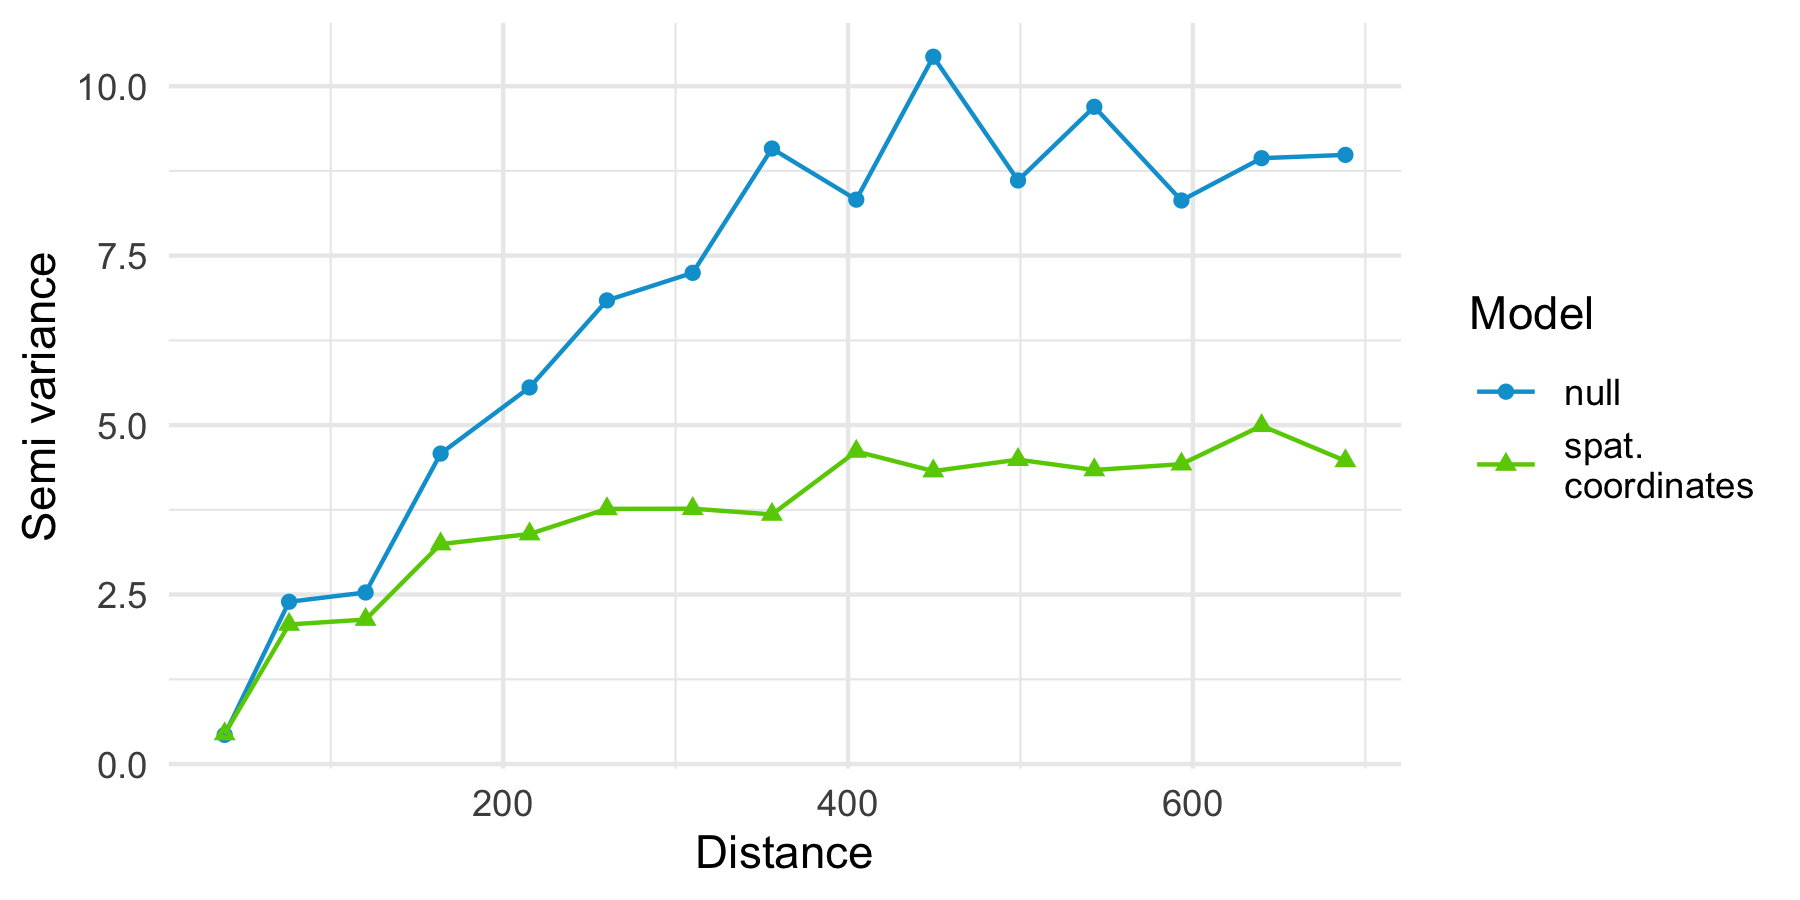
\includegraphics[width=10cm]{figs/variogram.png}
\caption{Variogram of the species Trisopterus esmarkii (Norway pout) from the Barents dataset with and without adjusting linearly for the spatial coordinates.}
\label{vario}
\end{figure}
However such correction might not be enough and the residuals from the adjustment might still be spatially correlated. Spatial coordinates could be adjusted in a more complicated way than the linear relationship, but another solution is to consider this dependence to be the result of an unobserved variable. As a missing variable, the spatial dependency can be taken into account to unravel the direct dependencies among species by using the method detailed in Chapter 3. Adjusting for spatial covariates corrects for the spatial effects on the means, whereas including spatial dependence  as a node in the interaction network corresponds to a correction of the variances.

%These two solutions aim at correcting for the spatial effect, which is thus considered as a kind of noise on the signal of species dependencies. However, one might be interested in modeling this spatial effect for further study. 

Another way of correcting the variances for spatial dependencies is to include spatial variances directly in the model. To do this a first approach is to assume a separation of the dependencies due to the spatial effects stored in the matrix $\Gamma=(\Gamma_{st})_{1\leq s,t\leq n}$ on the one hand, and due to the species interactions stored in the matrix $\Sigma=(\sigma_{jk})_{1\leq j,k\leq p}$ on the other hand. To simplify we consider either pairs of species $j$ and $k$ on the same site $s$ or a same species $j$ on pair of sites $s$ and $t$. The Gaussian parameters are then modeled as follows:
\begin{align*}
(Z_{sj},Z_{sk}) &\sim \Ncal(0, \gamma_{ss} \Sigma_{[j,k]}),\\
(Z_{sj},Z_{tj}) &\sim \Ncal(0, \sigma_{jj} \Gamma_{[s,t]}).
\end{align*}

That way we obtain $\Cov{(Z_{sj},Z_{sk})} = \gamma_{ss} \sigma_{jk}$ and $\Cov{(Z_{sj},Z_{tj})} =  \sigma_{jj}\gamma_{st}$. This is equivalent to consider the transformation of the matrix $\Zbf$ into the vector $Vec(\Zbf) = (Z_{11},..., Z_{1p},Z_{21},...,Z_{np}) \in \mathds{R}^{n\times p}$ to be distributed as:
$$Vec(\Zbf) \sim \Ncal(0,\Gamma \otimes \Sigma).$$ 

As the covariance structure is different for a pair of sites or a pair of species, this model requires to use the bivariate Poisson log-normal distribution for the count data $\Ybf$.
It is then possible to write a pairwise composite log-likelihood which involves all the variance parameters:
$$c\ell_\theta(\Ybf) = \sum_{j=1}^p \sum_{s<t} \log p_\theta(Y_{sj}, Y_{tj})+\sum_{s=1}^n \sum_{j<k} \log p_\theta(Y_{sj}, Y_{sj}).$$

The number of parameters for the variance is $\frac{1}{2}(n^2+ p^2)$, which is quite large. Classically to reduce this number, the $\Gamma$ matrix is parametrized with a spatial covariance function.  For example the Matérn functions (which include the exponential covariance function and others) define the covariance between two points distant of $d$ units from each other as a function of $d$ and three other parameters \citep{CW15}.

Performing network inference using tree averaging in this case would simply amount to consider 
$$Vec(\Zbf) \sim \Ncal(0,\Gamma \otimes \Sigma_T),$$
then the inference of edges probabilities would go as previously detailed.
 
%ovaskainen hmsc fait le job, à vérifier

\section{Network inference in the observed layer}
All of the above is an adaptation of the presented model to perform network inference in the latent Gaussian layer of parameters.
 However it can be shown that if the graphical model in the latent Gaussian layer $\Zbf$ is a connected graph, then the marginal graphical model of the observed counts $\Ybf$ is a clique. 
\begin{figure}[H]
\centering
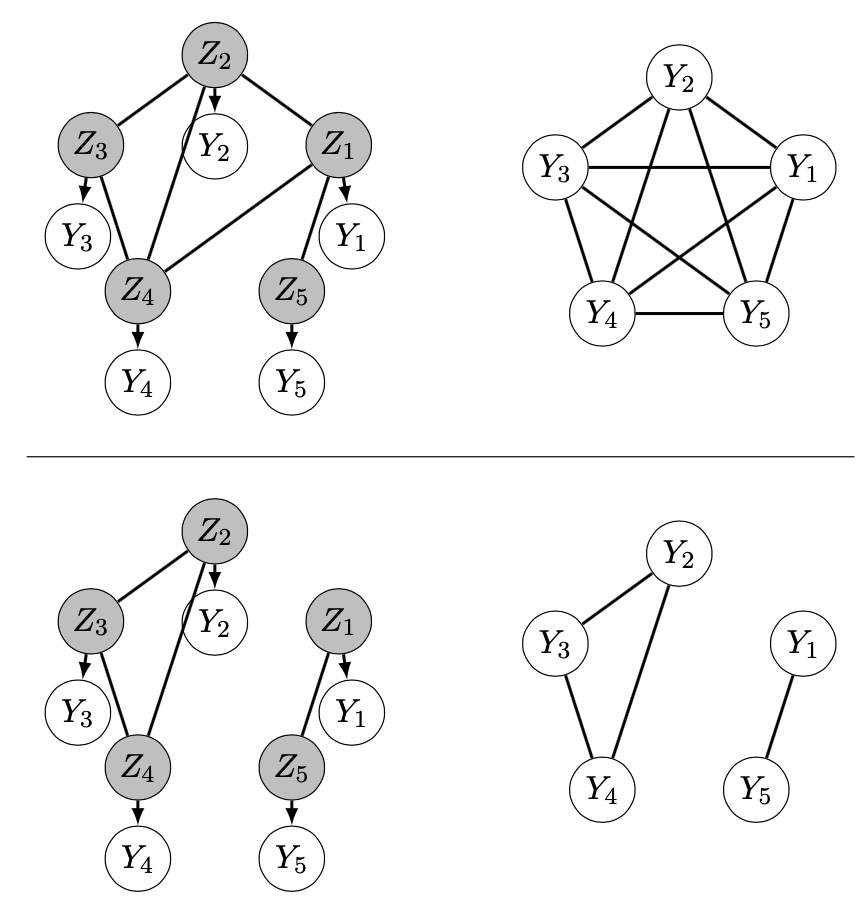
\includegraphics[width=0.5\linewidth]{figs/YZ.png}
\caption{Graphical representation of the joint distribution $p(Z_i,Y_i)$ (left) and marginal distribution $p(Y_i)$ (right) when the graphical model of the latent variables is connected (top) or not (bottom).}
\label{YZ}
\end{figure}
As Figure \ref{YZ} illustrates, only a separation in the latent space results in a separation in the observed space.


It is possible to write a model which meets the primary goal of inferring  the network directly in the space of observed data $\Ybf$. Considering any marginal and bivariate discrete distribution for counts, assuming a tree-shaped dependency structure for the counts writes: %it is possible to write the following model for the network inference using tree averaging:

 $$p_\theta(\Ybf_i \mid T) = \prod_{j=1}^p p_\theta(Y_{ij}) \prod_{jk\in T} \frac{p_\theta(Y_{ij},Y_{ik})}{p_\theta(Y_{ij})p_\theta(Y_{ik})}.$$
 
Covariates and offsets could be involved as parameters on the distributions means. Then the joint distribution of counts would be a mixture on trees:
$$p_{\beta, \theta}(\Ybf ) = \sum_{T\in \mathcal{T}} p_\beta(T)p_\theta(\Ybf\mid T).$$

This model involves only one latent layer: the tree $T$. With a decomposable distribution on $T$, the quantity $\Esp_{\beta, \theta}[\log p_{\beta, \theta}(\Ybf, T)\mid\Ybf]$ of the E step of an EM algorithm could be estimated using the Matrix Tree Theorem. Regarding the M step, the estimation of the weights $\beta$  would be the same as for the PLN model with network inference in the Gaussian layer. However the estimation of the $\theta$ parameter is complex, as its estimator is usually not explicit and is common to several terms of the product on the edges in $p_\theta(\Ybf\mid T)$. The M step is thus the main difficulty for the estimation of this model.
